\subsection{Проверка "<1С Розница"> на готовность к выгрузке}
%\marginnote{\Date{Вт.}{07}{Апр.}{2017}}[-40pt]
\begin{itemize}	
	\item Перед началом выгрузки данных из «Розницы» в «УТ» необходимо в «Рознице» запустить обработку - «КонтрольВыполненияРегламента.epf».
	 Рис.~\ref{ris:1.jpg}	
	\begin{figure}[H]
		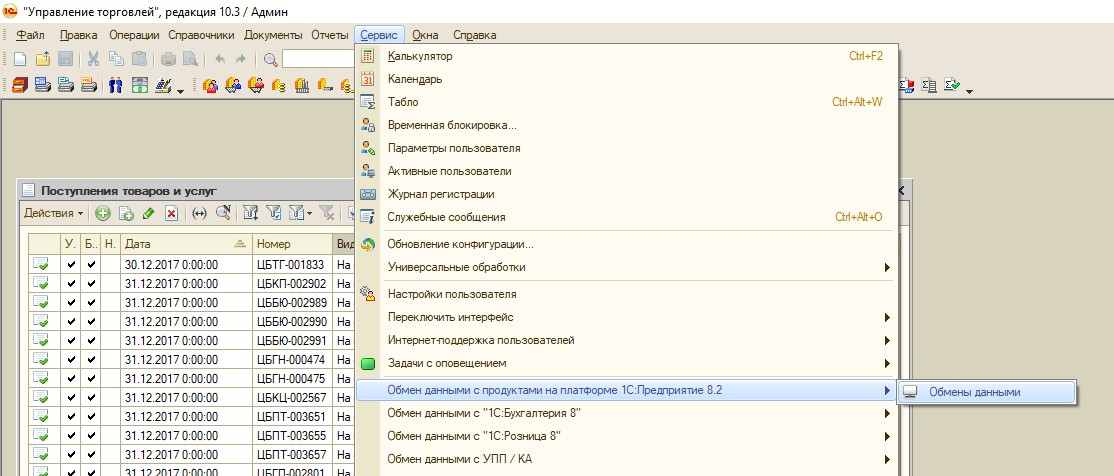
\includegraphics[width=0.8\textwidth]{1.jpg}
		\caption{Обработка контроля выполнения регламента выгрузки.}
		\label{ris:1.jpg}
	\end{figure}
Дата проверки указывается последним днем месяца выгрузки. После выполнения проверки, пустая колонка «Результат» будет указывать на пункты не прошедшие тестирование. Пункты прошедшие проверку буду обозначены зелеными "<галочками">.
 Рис.~\ref{ris:2.jpg}	
	\begin{figure}[H]
		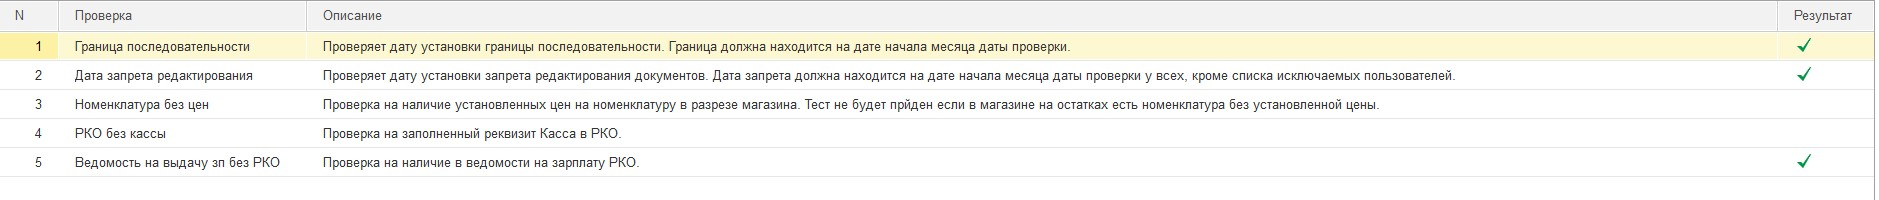
\includegraphics[width=0.8\textwidth]{2.jpg}
		\caption{Результаты тестирования.}
		\label{ris:2.jpg}
	\end{figure}
При двойном клике на строчке в колонке «Описание» если предусмотрено алгоритмом появиться список ошибок по этому пункту.
 Рис.~\ref{ris:3.jpg}
	\begin{figure}[H]
		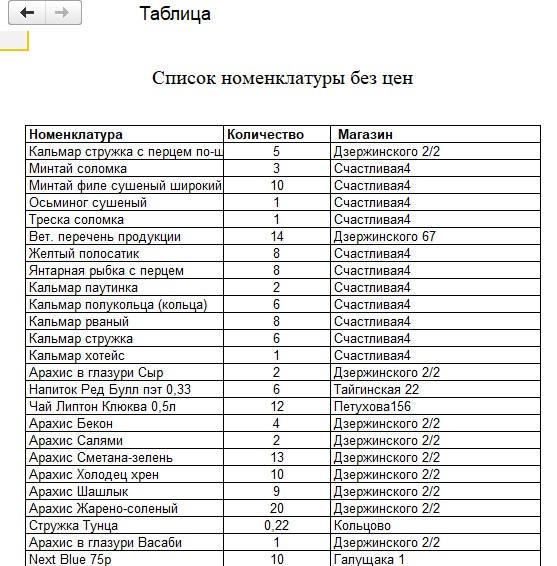
\includegraphics[width=0.39\textwidth]{3.jpg}
		\caption{Детализация по ошибкам.}
		\label{ris:3.jpg}
	\end{figure}
%\lstinputlisting[language=Python, firstline=7, lastline=45]{	echobot.py}
\emph{\color{Emerald}Заполнить выдачу зарплаты}
\todo{Добавить описние обработки по заполнению документов выдачи зарплаты}\par
После исправления ошибок,  нужно снова запустить проверку и убедиться в корректности исправлений. 
Когда тестирование будет пройдено без ошибок, можно приступать к выгрузке данных из "<1С Розница">
	
\end{itemize}
